\documentclass[10pt, onecolumn]{article}
 \usepackage{color,multirow,multicol}
 \usepackage{amsmath, amssymb, amsthm}
 \usepackage{calc,geometry,mathrsfs,xspace,graphicx,hyperref}
 \usepackage{subfig}

 \setlength{\evensidemargin}{0.0in}
\setlength{\oddsidemargin}{0.0in} \setlength{\textwidth}{6.5in}
\setlength{\topmargin}{-0.5in} \setlength{\textheight}{9in}
% type user-defined commands here

  \makeatletter
 \DeclareRobustCommand\onedot{\futurelet\@let@token\@onedot}
 \def\@onedot{\ifx\@let@token.\else.\null\fi\xspace}
 \newcommand{\R}{\mathbb{R}}
 \newcommand{\Li}{\mathcal{L}}
 \newcommand{\1}{\textbf{1}}
 \newcommand{\err}{\epsilon}
  \def\etal{\emph{et al}\onedot}

\title{Larva Behavior Labeling Tool}
\author{Steve Branson\\sbranson@cs.ucsd.edu 
\and Kristin Branson\\bransonk@janelia.hhmi.org}

\begin{document}
\maketitle

\section{Introduction}

The larva behavior labeling tool is a tool for annotating, training, and detecting larva behaviors and annotating and fitting larva skeletons.  The basic tool is depicted in Figure \ref{fig:screenshot}.

\begin{figure}[t]
\centering
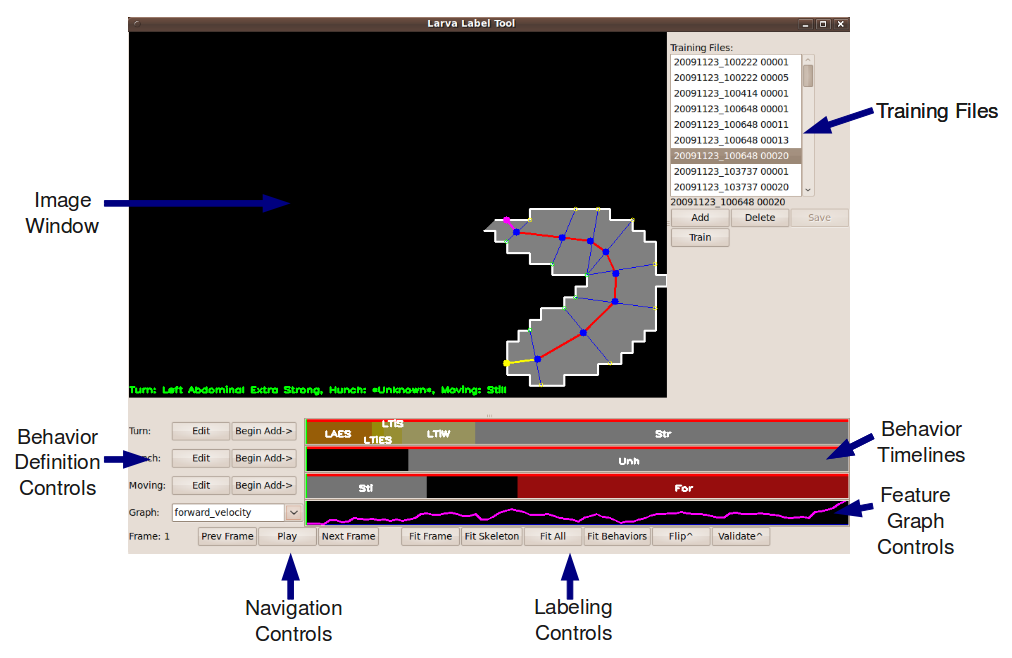
\includegraphics[width=17.0cm]{Screenshot.png}
\caption{Screenshot of the Larva Behavior Labeling Tool}
\label{fig:screenshot}
\end{figure}

\section{Installation and Compilation}

The tool was developed and tested mostly on Ubuntu 9.10 64-bit Linux, and had been compiled and run (but not thoroughly tested) on Windows 7 and Mac OS X Snow Leopard.  

\subsection{Running the Tool}
Obtain the package by emailing Steve (sbranson@cs.ucsd.edu), or by downloading using SVN (see \ref{sec:svn}).  The package should contain a folder called \textit{larva} with a bunch of subfolders (like \textit{code, doc, data, windows, mac}).
\begin{itemize}
 \item \textbf{Windows: } Double click the file \textit{gui.exe} in the folder \textit{larva/windows}
 \item \textbf{Mac: } Double click the file \textit{run} in the folder \textit{larva/mac}
 \item \textbf{Linux: } From a terminal, type \textit{./gui} from the folder \textit{larva/code}
\end{itemize}
If this doesn't work, please email Steve (sbranson@cs.ucsd.edu) with a description of what happened and any error messages that appear.  It is highly possible that I forgot to include some necessary libraries to run on some versions of for Mac or Windows.

\subsection{Running and Compiling From the Source Code}
You can also obtain the tool's source code and use that to compile an executable and run the tool.  This is currently the preferred method of running the tool, because I am still making changes to it and you will be able to run the latest version of the tool.

\subsubsection{Downloading the Source Code Using SVN}
\label{sec:svn}
SVN is a revision control system that makes it easier for multiple developers work on the same code, by tracking and maintaining different versions and changes to the code.

\begin{itemize}
 \item \textbf{Step 1: } Check out the SVN repository.  \textbf{This is a one time thing}, and is basically how you download all the larva code and data initially.  If you have done this already, proceed to Step 2.
 \begin{itemize}
   \item \textbf{Mac:} \begin{itemize}
     \item Open a terminal (located in /Application/Utilities).  
     \item Navigate to the folder where you want to put the code (you can type the command \textit{cd folder\_name} to enter the directory \textit{folder\_name}). 
     \item Check out the repository by typing \\ \textit{svn checkout https://subversion2.int.janelia.org/branson/projects/larva} (you must be connected to the Janelia network).  If it succeeds, it should create a directory called \textit{larva}, and you should see it print out a list of files as they are downloaded.  
     \item If you get an error to the effect of ``svn doesn't exist'', you can install svn by following Steps 1-3 at http://www.wikihow.com/Install-Subversion-on-Mac-OS-X
   \end{itemize}
   \item \textbf{Windows: } \begin{itemize}
     \item If you don't have an SVN client, you can install Tortoise SVN: \url{http://tortoisesvn.net/downloads}.  
     \item Use a file browser to go to the directory where you want to put the code.  
     \item Right-click, you should see a Windows menu popup.  Select the menu option \textit{SVN Checkout}.  
     \item In the field \textit{URL of repository} enter\\ \textit{https://subversion2.int.janelia.org/branson/projects/larva} (you must be connected to the Janelia network), then press \textit{Ok}.  If it succeeds, it should create a directory called \textit{larva}, and you should see it print out a list of files as they are downloaded. 
   \end{itemize}
   \item \textbf{Linux: } Same as Mac, except that if you don't have SVN, install the package \textit{subversion} (e.g., \textit{sudo apt-get install subversion})
 \end{itemize}
 \item \textbf{Step 2: } Get the latest version of the code.  \textit{Note: } you must be connected to the Janelia network.
   \begin{itemize}
   \item \textbf{Mac:} From a terminal (located in /Application/Utilities), navigate to the folder 'larva' (e.g., \textit{cd folder\_name}), which was created using the previous step.  Type \textit{svn update}
   \item \textbf{Windows:} From a file browser, right-click on the folder \textit{larva} (created using the previous step).  A windows menu should popup, select \textit{SVN Update}
   \item \textbf{Linux: } Same as Mac
 \end{itemize}
\end{itemize}

\subsubsection{Compiling and Running the Source Code}
After following the steps in Section \ref{sec:svn}, you should have a folder names \textit{larva} and can compile the code into an executable.  If it works it's pretty easy.  If you get errors, email Steve (sbranson@cs.ucsd.edu) with a description of what happened and any error messages that appear.

\textit{Note:} The code has 2 main library dependencies: wxWidgets and OpenCV.  For Mac OS X, I tried to package these libraries inside \textit{larva/mac\_local}, which worked on Wyatt's laptop; however I'm not $100\%$ sure it will work on other computers.
\begin{itemize}
  \item \textbf{Mac:} \begin{itemize}
    \item Open a terminal (located in /Application/Utilities).  
    \item Navigate to the folder \textit{larva/code}  (e.g., type \textit{cd larva/code})
    \item Set the library path by typing \textit{export DYLD\_LIBRARY\_PATH=../mac\_local/lib}
    \item Type \textit{make} to compile the code.  If it succeeds, you should see a bunch of lines printed like \textit{g++ -g -Wall...}, and it will generate an executable file \textit{larva/code/gui}.
    \item Run the larva labeling tool by typing \textit{./gui}
  \end{itemize}
  \item \textbf{Windows:} \begin{itemize}
    \item Open the project file \textit{/larva/code/larva.sln} (Requires the Microsoft Visual C++ compiler)
    \item Make sure you have installed OpenCV \url{http://opencv.willowgarage.com/wiki/VisualC\%2B\%2B}) and wxWidgets (\url{http://wiki.wxwidgets.org/Microsoft_Visual_C\%2B\%2B_Guide}
    \item Select the menu option \textit{Build $\to$ Build Solution} to compile the code.  If it succeeds, it should print a line \textit{===Build: 1 succeeded} in the output log, and it will generate an executable file \textit{larva/windows/gui.exe}.
    \item Open the file \textit{larva/windows/gui.exe} to run the labeling tool
  \end{itemize}
  \item \textbf{Linux:} Same as Mac.  Make sure you have wxWigets \\(\textit{sudo apt-get install build-essential libwxgtk2.8-dev libwxgtk2.8-dbg}) and OpenCV (\url{http://opencv.willowgarage.com/wiki/})
\end{itemize}

\section{User Guide}

\subsection{Opening/Importing/Removing Files}
\label{sec:open}
\begin{itemize}
 \item \textbf{Opening a File:} Open a larva file for annotating by clicking an entry in the \textit{Training Files} listbox.
 \item \textbf{Importing a File:} To add a file not yet in the \textit{Training Files} listbox, click the \textit{Add}, browse for a .outline larva contour file (as outputted by Rex's tracker), then click \textit{Open}.  The file should be added to the bottom of the \textit{Training Files} listbox.  Files inside this list will be used to train the Behavior Detector.  
 \item \textbf{Removing a Training File:} To remove a file from this list, click the \textit{Delete} button.  This removes the file from the training file list, but does not physically delete the file.
\end{itemize}

\subsection{Detecting Behaviors and Fitting Skeletons}
\label{sec:detect}
Once you have opened a larva file (Section \ref{sec:open}), you can try to automatically fit a skeleton to each larva contour in the tracked sequence and detect the corresponding sequence of larva behaviors.  This is done using the Fit buttons in the \textit{Labeling Controls} panel.  The skeleton is a curve passing through the center of the larva from the tail to the head.  It is depicted as a series of red line segments in the \textit{Image Window}.  There are 3 predefined groups of behaviors: \textit{Turn}, \textit{Hunch}, \textit{Moving}.  Each behavior group is displayed and labeled independently (there are 3 different timelines in the \textit{Behavior Timelines}).  Each behavior group has a collection of mutually exclusive behavior classes, e.g. \textit{Left Thoracic Weak, Right Tip Strong, Straight}, etc.  The behaviors are depicted in the \textit{Behavior Timelines} as a sequence of colored bars (see Figure \ref{fig:behaviors}).

The \textit{Fit All} button will detect both the skeleton and the behavior sequence, whereas \textit{Fit Skeleton} and \textit{Fit Behaviors} will detect only one or the other.  You cannot detect behaviors unless a detected skeleton already exists (either using \textit{Fit Skeleton}, \textit{Fit All}, or stored in an existing annotation file if you have edited this larva file before).  You should be able to see the results of a fit skeleton and/or behavior sequence in the \textit{Image Window} and \textit{Behavior Timelines}.

\subsection{Viewing and Navigating Around Larva Blob Sequences}
Once you have opened a larva file (Section \ref{sec:open}), an image should appear in the \textit{Image Window} which shows the larva blob for frame 1 of the tracked blob sequence.  A tracked blob sequence corresponds to a particular larva animal over some period of time $t=1...T$, as returned by Rex's tracker.  The \textit{Behavior Timeline} controls are used to represent this period of time, where the leftmost part of the timeline corresponds to the first frame $t=1$ and the rightmost part corresponds to $t=T$.  Hovering the mouse over a portion of the timeline will draw the larva blob of the corresponding time in the \textit{Image Window}.  Clicking a point in the timeline will set the current frame to the corresponding point, visualized using a vertical green bar (see Figure \ref{fig:time}).  The buttons \textit{Prev Frame} and \textit{Next Frame} will change the current frame to one frame earlier and one frame later, respectively.  Pressing the \textit{Play} button will play the blob sequence in real time.  You will need to press the \textit{Play} button again to pause/stop the play animation.

\subsection{Annotating Behaviors}

To add a new behavior bout, follow the steps outlined in Figure \ref{fig:add_behavior}.  Press the \textit{Save} button near the \textit{Training Files} list to save changes to the currently opened larva blob sequence.

\begin{figure}
 \subfloat[Select a file to annotate by clicking an entry in the \textit{Training Files} listbox.]{\label{fig:select}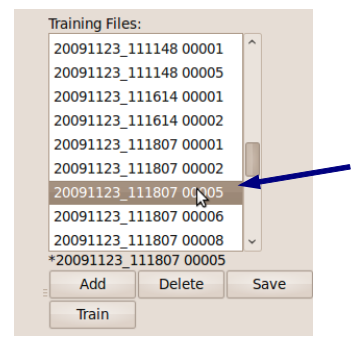
\includegraphics[height=5cm]{SelectFile.png}}   
 \quad \subfloat[Click on the \textit{Behavior Timeline} at the time frame when your behavior starts.]{\label{fig:time}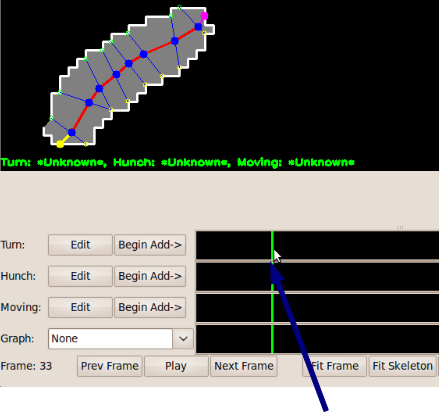
\includegraphics[height=5cm]{ClickTimeline.png}}  
 \quad \subfloat[Click on the \textit{Begin Add} button next to the behavior group you want to add a behavior for (in this case \textit{Turn}).]{\label{fig:begin_add}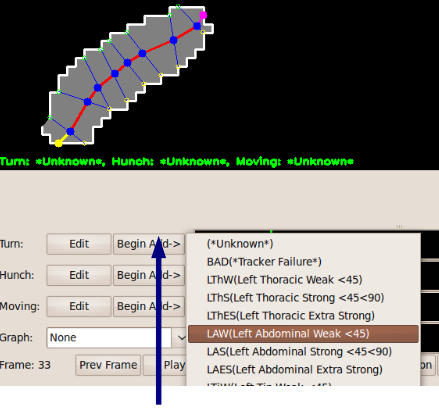
\includegraphics[height=5cm]{BeginAdd.png}} 
 \\ \subfloat[Move your mouse over the \textit{Behavior Timeline} to the frame when your behavior ends. A green highlighted region should appear.]{\label{fig:end_hover}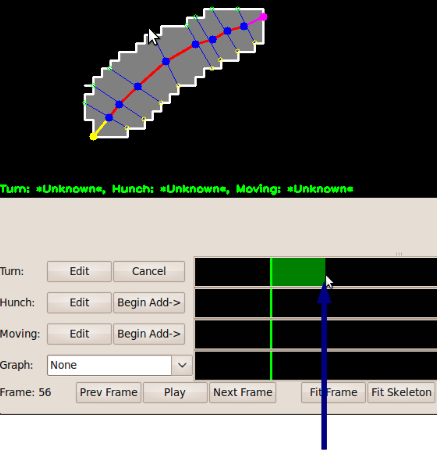
\includegraphics[height=5.5cm]{EndBehavior.png}} 
 \quad \subfloat[Click the mouse to finish adding your behavior.  The new behavior should appear on the timeline.]{\label{fig:end_finish}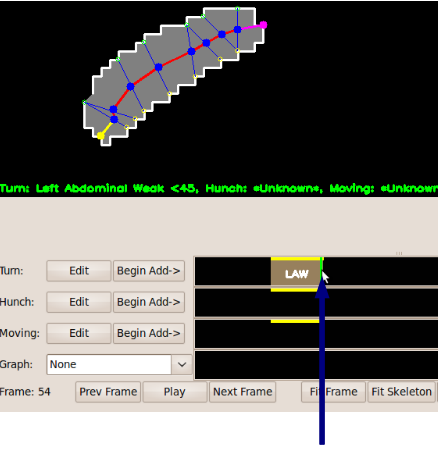
\includegraphics[height=5.5cm]{EndBehavior2.png}} 
\label{fig:add_behavior}
\caption{\textbf{Adding a New Behavior Bout:} The example above depicts the sequence of steps used to add a new behavior bout for \textit{Turn Left Abdominal Weak}.}  
\end{figure}

\subsection{Annotating Skeletons}

\begin{minipage}[b]{1.0\linewidth}
\centering
\begin{minipage}[b]{0.3\linewidth}
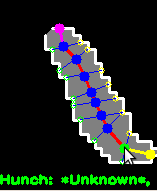
\includegraphics[height=5cm]{EditSkeleton.png}
\end{minipage}
\begin{minipage}[b]{0.5\linewidth}
In general, you should just use the automatic skeleton fitting routines (Section \ref{sec:detect}); however, it is also possible to adjust the skeleton location manually.  This can be done by clicking and dragging one of the blue skeleton points in the \textit{Image Window}, which should appear in green when you place the mouse over it. Press the \textit{Save} button near the \textit{Training Files} list to save changes to the currently opened larva blob sequence.
\end{minipage}
\end{minipage}

\subsection{Verifying Annotations}
\label{sec:verify}

Since it is possible for the computer to automatically predict both the skeleton and the behavior, a human has to verify the correctness of the predicted skeleton/behavior before that data can be considered to be good training data (for training a better behavior detection algorithm).  A frame is automatically marked as verified if it was labeled manually.  The procedure for verifying a sequence of frames as correct is similar to the procedure for labeling behaviors in Figure \ref{fig:add_behavior}, except that the \textit{Verify} button is used instead of the \textit{Begin Add} button.  In other words, click on the timeline the starting frame of the sequence you want to verify, then click the \textit{Verify} button, then click on the timeline the ending frame of the sequence you want to verify.  Verified frames will be displayed with a bright red strip on the top of the timeline.  Frames where the skeleton has been verified but not the behavior are drawn in magenta, and frames where the behavior has been verified but not the skeleton are drawn in yellow.  Only bright red frames (where both the skeleton and behavior have been verified) are used for training.  Press the \textit{Save} button near the \textit{Training Files} list to save changes to the currently opened larva blob sequence.

\hspace{-.8cm}
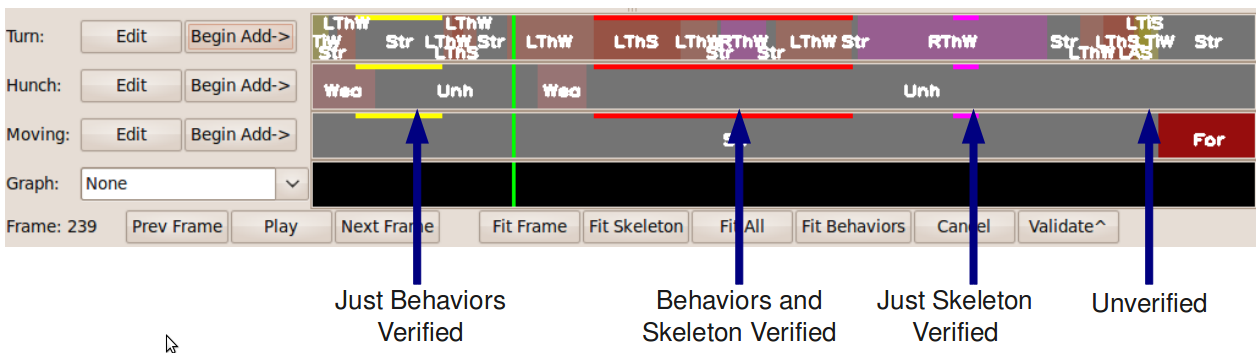
\includegraphics[width=17cm]{Verify.png}

\subsection{Training the Behavior Detector}
\label{sec:train}

After you have annotated some larva blob files, you can train a behavior detector by pressing the \textit{Train} button near the \textit{Training File} listbox.  The learning algorithm will learn from any frames in files in the training list that have been verified and highlighted in bright red (see \ref{sec:verify}).  Training may take on the order of hours to complete.  After training finishes, the \textit{Fit Behavior} button can be used to apply the learned detector to a larva blob sequence. Some tips on constructing a good training set are:
\begin{itemize}
 \item Try to label at least 10-20 larva files
 \item Make sure the larva files that you annotate are representative of the larva files that you want the system to work on.  In other words, if the annotated larvae come from a different experiment where the larvae appear very different, the learned behavior detector won't behave very well.
 \item Make sure you get a lot of example sequences for every type of behavior.  For example, only having one annotated bout of some rare behavior (e.g. \textit{Sigmoidal left to right}) might cause that behavior detector to be very unreliable.  It is best to have at least 10-20 labeled examples of each type of behavior.
 \item If possible, label or verify all frames in a given larva blob sequence (as opposed to verifying some frames in a particular file while leaving some other frames unverified)
 \item There are 2 special ``behaviors'' added by default \textit{Unknown} and \textit{Tracker Failure}.  The label \textit{Unknown} pretty much means ``don't care'' or ``can't tell'', e.g. it doesn't really matter what these frames are labeled as.  The label \textit{Tracker Failure} should be used when the larva blob contour was bad (e.g. the shape of the detected blob is very different from the shape of a real larva, due to a tracking problem), such that the skeleton fit was bad.
 \item If you train on a machine with multiple processors/cores, it will run faster
\end{itemize}


\subsection{Changing the Behavior Definitions}

You can alter the list of the types of behaviors, e.g. \textit{Turn Left Tip Strong}, either adding new behaviors, deleting old ones, or renaming old ones.  On the other hand, you should be careful about doing this because behavior annotation files depend on the defined list of behaviors such that changing the list of behaviors may invalidate them.  Any files relating to learned behavior detectors will almost certainly be invalidated (you may need to manually remove files in \textit{larva/data/classifier} to avoid errors).  As a result, it's a good idea to just edit behaviors once, before you start annotating files, and then not change them again.  If you still want to edit the behavior definitions, it's a good idea to backup your files first (see Section \ref{sec:backup}).

You can edit behaviors by clicking on the \textit{Edit} button in the \textit{Behavior Definition Controls}, which should open up a window with the list of available behaviors.  Use the \textit{Add}, \textit{Edit}, \textit{Delete} buttons to alter the list of behaviors as desired.  It's pretty straightforward what these controls do.  The one non-obvious option is the \textit{Color} field when editing a particular behavior.  This is the color that is used to draw the behavior in the timeline controls, defined in hexadecimal 0xRRGGBB, where RR is the red component, GG is thre green component, and BB is the blue component (see \textit{http://www.computerhope.com/htmcolor.htm}).  Any changes you make will not take effect until you select the \textit{Save} button.

There is currently no mechanism in the GUI for defining new Behavior groups (e.g. Turn, Hunch, Moving); however, you can probably do this by editing the file \textit{larva/data/behaviors.txt}.  Changes made to this file should show up in the GUI.

\subsection{Backing Up Files}
\label{sec:backup}

It might be a good idea to backup files before you make any changes to the behavior definitions or training file list, since changing the behavior definitions can invalidate existing annotations. You can backup all configuration and annotation data files (all files described in Section \ref{sec:data}) by clicking the \textit{Backup} button under the \textit{Training Files} listbox.  This will create a directory \textit{larva/backup/backup\_timestamp}, where \textit{backup\_timestamp} is the current time/date.  You can run the label tool GUI using the backed up files (this will both read in the backed up files and save new annotation changes to the backed up files) by running starting the label tool with the command line arguments: \textit{./gui -d ../backup/backup\_timestamp}.

\section{Data Files}
\label{sec:data}

Data files are stored in the folder \textit{larva/data}.  The most important configuration related data files (you should consider backing these up before you make any major changes) are:
\begin{itemize}
 \item \textit{larva/data/train.txt}: contains the list of larva blob data files that are used for training the behavior detector and are selectable \textit{Training Files} listbox in the GUI.  This file gets edited when you Add/Delete files in the \textit{Training Files} listbox. 
 \item \textit{larva/data/behaviors.txt}: contains the definition of behaviors that are detectable and annotatable.  These are editable in the GUI in the \textit{Behavior Definition Controls} and annotatable in the \textit{Behavior Timelines}.  This file gets edited when you Add/Edit/Delete behaviors in the \textit{Behavior Definition Controls}.
 \item \textit{larva/data/classifier/All.svmbehavior}: contains the data files for the learned behavior detector.  This is generated when the user trains the behavior detector via the \textit{Train} button.
\end{itemize}

The data files containing annotations for individual animals are stored in the folders like \textit{larva/data/20091123\_100222}.  These are direct copies of data folders that were generated from Rex's Multi Worm Tracker.  The Larva Behavior Tool imports files like\\
\textit{larva/data/20091123\_100222/20091123\_100222@w1118@n@t1@p\_strongside\_15s1x30s0s\#n\#n\#n@1@.00001.outline}, which contain the contours of tracked larva blobs and are generated by Rex's tracker.  It outputs files like\\
\textit{larva/data/20091123\_100222/20091123\_100222@w1118@n@t1@p\_strongside\_15s1x30s0s\#n\#n\#n@1@.00001.anno}.  The \textit{.anno} files contain all information stored in the \textit{.outline} files, as well as information relating to the detected or annotated larva skeleton, and detected or annotated larva behaviors.





\end{document}

